\section{微积分基本定理-上}\label{018}

\begin{tcolorbox}[size=fbox, breakable, enhanced jigsaw, title={微积分基本定理 (fundamental theorem of calculus)}]

前面只讲了积分的动机和定义, 但是并没有涉及具体的运算,
那么这里先摆出结论: 积分和微分可以视作互逆的运算.
这一点在很多高中的教材似乎是默认的, 但是事实上真的如此吗?
为了证明这一点, 首先, 令 \[
F(x):=\int_a^xf(\xi)\mathrm{d}\xi,
\]

\begin{newquote}
怎么突然出现了 \(\xi\) ? 其实原则上写 \(f(x)\mathrm{d}x\)
也没有太大问题, 但是积分的上限也是 \(x\), 为了加以区分,
所以将积分对象的变量改为其他字母, 其含义是没有发生任何变化的
(参见【\ref{017}\nameref{017}】对于 dummy variable 的讨论). 只是积分对象和积分上限都用
\(x\) 有滥用标记 (abuse of notation) 之嫌, 不是非常专业.
\end{newquote}

考虑 \(F(x)\) 的斜率, 首先是近似的形式 \[
\begin{aligned}
&\frac{F(x+h)-F(x)}{h}\\
=&\frac{1}{h}\left(\int_a^{x+h}f(\xi)\mathrm{d}\xi-\int_a^xf(\xi)\mathrm{d}\xi\right)\\
=&\frac{1}{h}\int_x^{x+h}f(\xi)\mathrm{d}\xi.
\end{aligned}
\] 上式最后两行可以如下图所示地用函数下的面积来理解,
不难看出第一个积分得到的是深色面积,
第二个积分得到的是深色和浅色的面积之和, 于是他们的差便是浅色的面积,
浅色面积对应的区间是 \([x,x+h]\), 于是相当于是上下限分别是 \(x\) 和
\((x+h)\) 的积分.

\begin{tcolorbox}[size=fbox, breakable, enhanced jigsaw]
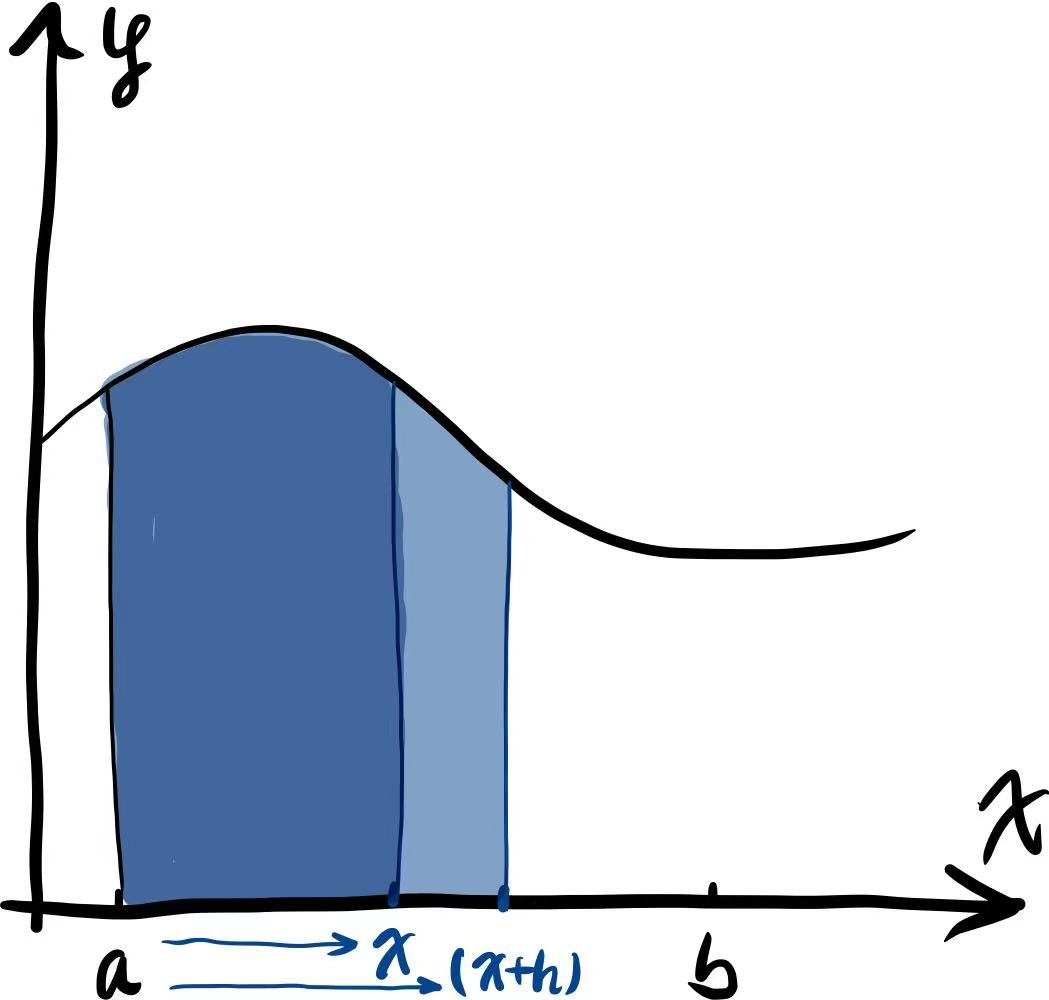
\includegraphics[width=0.3\textwidth]{img/image-20230912145204089.png}

\end{tcolorbox}

\begin{tcolorbox}[size=fbox, breakable, enhanced jigsaw, title={插曲: 定积分的中值定理}]\footnote{其实应该现有了微积分基本定理再推积分的中值定理会更方便,
  中值定理有 \(f'(c)=(f(b)-f(a))/(b-a)\) 对于某个区间 \([a,b]\) 内的
  \(c\). 令 \(F(x):=\int_a^xf(\xi)\mathrm{d}\xi\), 将 \(F(x)\)
  直接套入中值定理, 再利用积分和求导互为逆运算, 便有
  \(f(c)=F'(c)=(F(b)-F(a))/(b-a)\).}

若 \(f(x)\) 在区间 \([a,b]\) 连续, 则存在某点 \(c\) 使得, \[
\boxed{f(c)=\frac{1}{b-a}\int^b_af(x)\mathrm{d}x.}
\] 像 \(\frac{1}{b-a}\int_a^bf(x)\mathrm{d}x\) 这样的形式,
事实上是取了函数 \(f(x)\) 在区间 \([a,b]\) 的``平均值'', 即:
【把这个形式得到的值想象成高, 把 \([a,b]\) 想象成底,
相乘得到的矩形面积】和【积分对应的函数图像下的面积】应该是一致的;
那么自然, 这个``平均值''是小于这个区间内 \(f(x)\) 的最大值,
而大于这个区间内 \(f(x)\) 的最小值的; 同时, 因为 \(f(x)\) 是连续的,
那么必然在这个区间内存在至少一点 \(c\) 使得 \(f(c)\) 等于这个``平均值''.

\end{tcolorbox}

有了定积分的中值定理, 再对比一下前面 \(F(x)\) 的斜率的近似形式, 不难发现
\([x,x+h]\) 这个区间内, 也应该存在某点 \(c\), 使得
\(f(c)=\frac{1}{h}\int_x^{x+h}f(\xi)\mathrm{d}\xi\). 这里要注意, 这个
\(c\) 并不是固定的, 随着 \(h\) 的变化, \(c\) 应该也是随之变化的.

接下来的操作很不严谨的 (hand-wavy, 这边有一个很难直译的词,
当说一些很模棱两可又暧昧的说法时, 我们可能会习惯性地波动我们的手),
取极限 \(h\rightarrow0\) 是, 于是 \([x,x+h]\) 这个区间也越来越窄,
到最后迫使 \(f(c)\rightarrow f(x)\). 于是便有 \[
F'(x)=\lim_{h\rightarrow 0}\frac{1}{h}\int_x^{x+h}f(\xi)\mathrm{d}\xi=f(x).
\] 这便是\textbf{微积分基本定理} (fundamental theorem of calculus),
重新表述如下: \[
\boxed{\frac{\mathrm{d}}{\mathrm{d}x}\int_a^xf(\xi)\mathrm{\xi}=f(x).}
\] 可以看到, 一个函数经过积分又求导后变回了原函数,
可见微分和求导一定程度上确实应该是互为逆运算的. 这样,
当我们实际计算积分时可以利用\textbf{反导数 }(antiderivative) 来完成计算.

\begin{tcolorbox}[size=fbox, breakable, enhanced jigsaw, title={反导数}]

在某个区间内, 若对于任意 \(x\) 都有
\(F'(x)=\frac{\mathrm{d}}{\mathrm{d}x}F(x)=f(x)\), 则在此区间内函数
\(F(x)\) 是 \(f(x)\) 的反导数.

于是, 对于一个在区间 \([a,b]\) 内连续的函数 \(f(x)\), 它的定积分,
用微积分基本定理可以表述为: \[
\boxed{\int_a^bf(x)\mathrm{d}x=F(b)-F(a),}
\] 这里 \(F(x)\) 是 \(f(x)\) 在区间 \([a,b]\) 的反导数.

\end{tcolorbox}

\begin{newquote}
例: \(\int_a^b x\mathrm{d}x\)

我们知道, 求导时, 多项式的会先乘上次数, 然后次数会减一,
那么逆导数便应该是次数加一, 然后除以新的次数 (顺过来的运算后执行的,
逆运算先执行),

\begin{tcolorbox}[size=fbox, breakable, enhanced jigsaw]
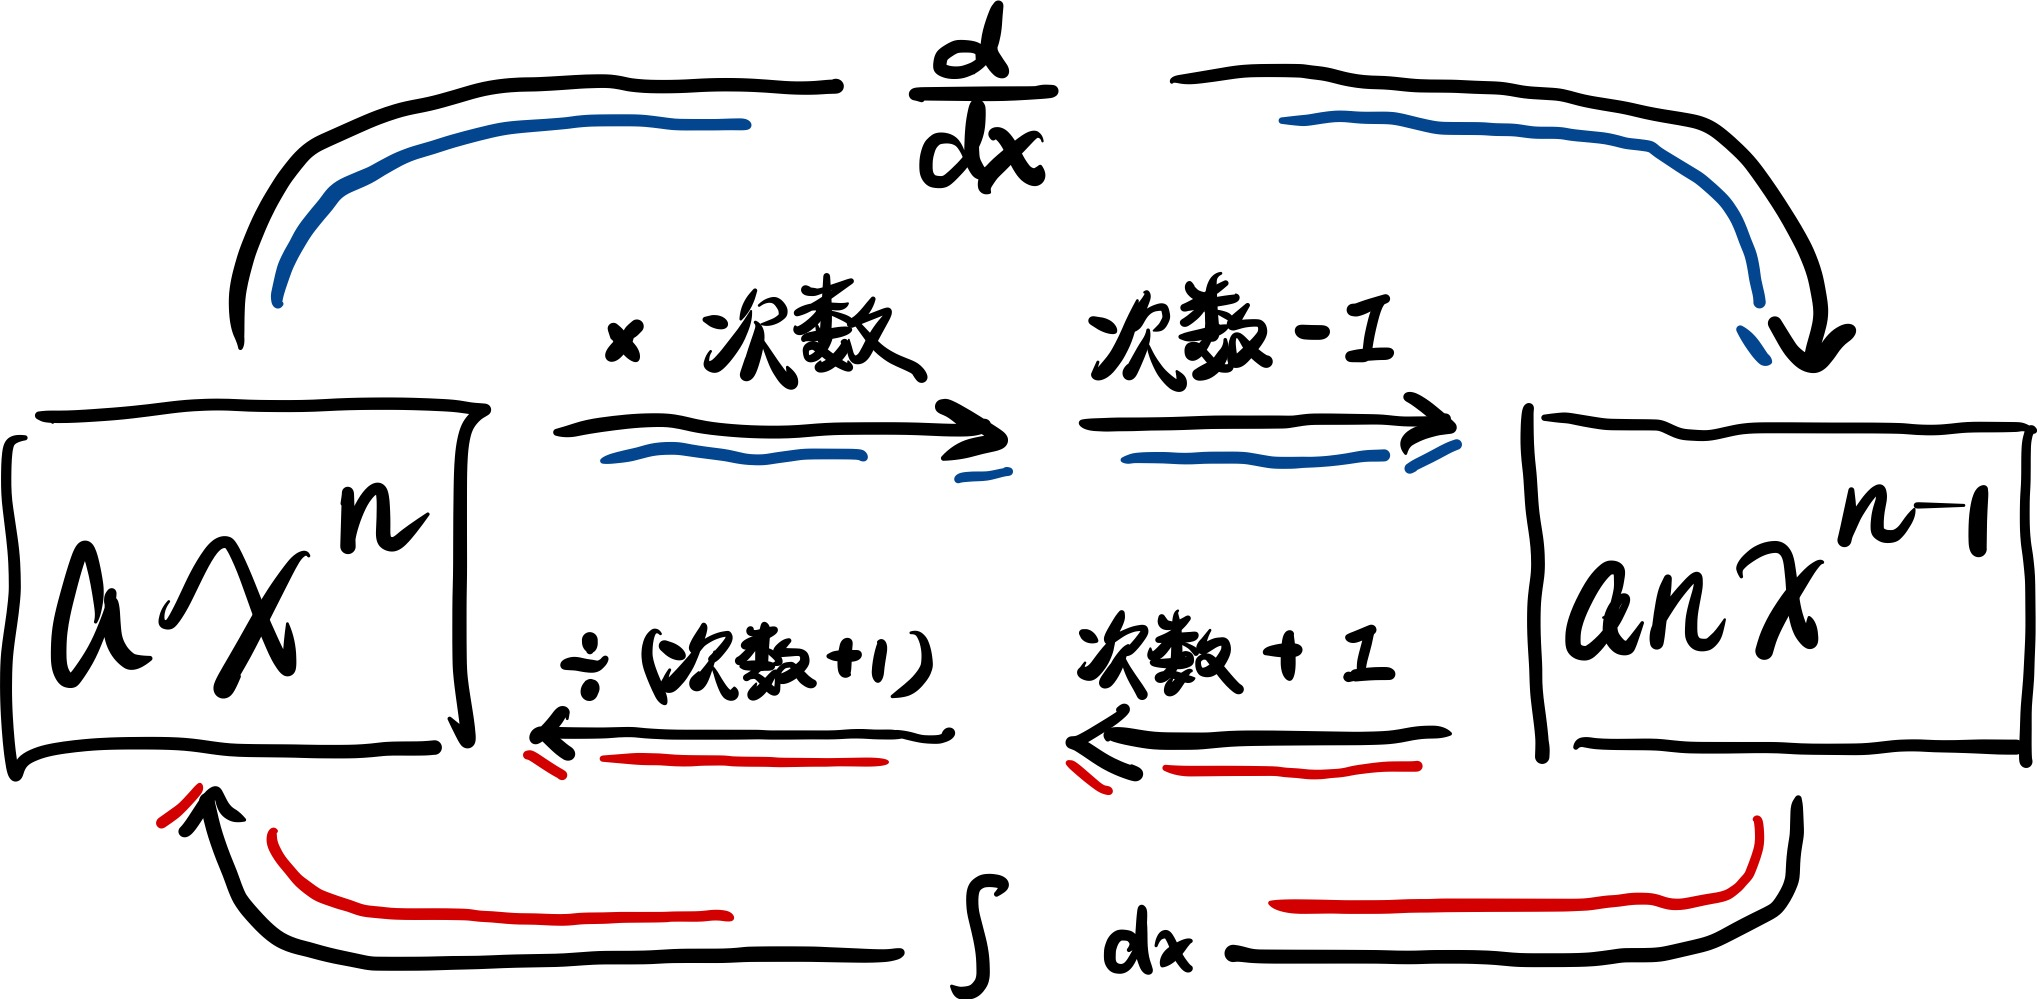
\includegraphics[width=0.6\textwidth]{img/image-20230912161734076.png}

\end{tcolorbox}

类似的, 三角函数, 指数函数, 对数函数, 符合函数 (复习链式法则,
参见【\ref{013}\nameref{013}】) 等等的逆导数也可以用这样的思路去求.

如此这般, 首先, 若 \(f(x)=x\), 应该对应逆导数 \(F(x)=\frac{1}{2}x^2\).
然后 \[
\begin{aligned}
  \int_a^bf(x)\mathrm{d}x&=F(b)-F(a)\\
  &=\frac{1}{2}b^2-\frac{1}{2}a^2.
\end{aligned}
\] 习惯上我们更通常这么写 \[
\begin{aligned}
\int_a^bx\mathrm{d}x=&\left.\frac{1}{2}x^2\right|_{x=a}^b\\
=&\frac{1}{2}b^2-\frac{1}{2}a^2.
\end{aligned}
\] 右边一竖的意思是在 \(x=a\) 和 \(x=b\) 处分别求值 (evaluate)
再求差的意思.
\end{newquote}

\begin{tcolorbox}[size=fbox, breakable, enhanced jigsaw, title={不定积分}]

前面积分时, 都强调了积分的上下限,
但是有的时候我们可能需要一个通常的表达式, 而不需要求值,
这种积分我们称作不定积分. 一个函数的不定积分等于它的逆求导加上一个常数:
\[
\int f(x)\mathrm{d}x=F(x)+\text{const.}
\] 等价的说法是, 一个函数其实并不只有一个逆导数,
但是这些逆导数只差了一个常数 (和积分变量无关). 这是因为求导时,
常数项直接``消失''了. 这就带来了规范自由 (gauge freedom)\footnote{超纲警告!
  规范自由本质上来说就是一个标量场加上一个常数并不会影响它的梯度.}.

\end{tcolorbox}
\end{tcolorbox}